To measure quantitative accuracy of our model, we took a video recording of each of our participants. We then manually counted the number of repetitions for each of the exercises in our routine and compared them to the count estimates given by our model. The figures below show our results as 100\% stacked column charts. If our model performed accurately, both the ''Actual'' and the ''Estimated'' bars would account for 50\% each. If the ''Estimated'' bar comprises less than 50\%, it means our model underestimated the total count; correspondingly, if the ''Estimated'' bar takes up over 50\%, it means our model overestimated. For reference, we also included a table detailing the counts under each of the graphs.\\
\begin{figure} [htp]
	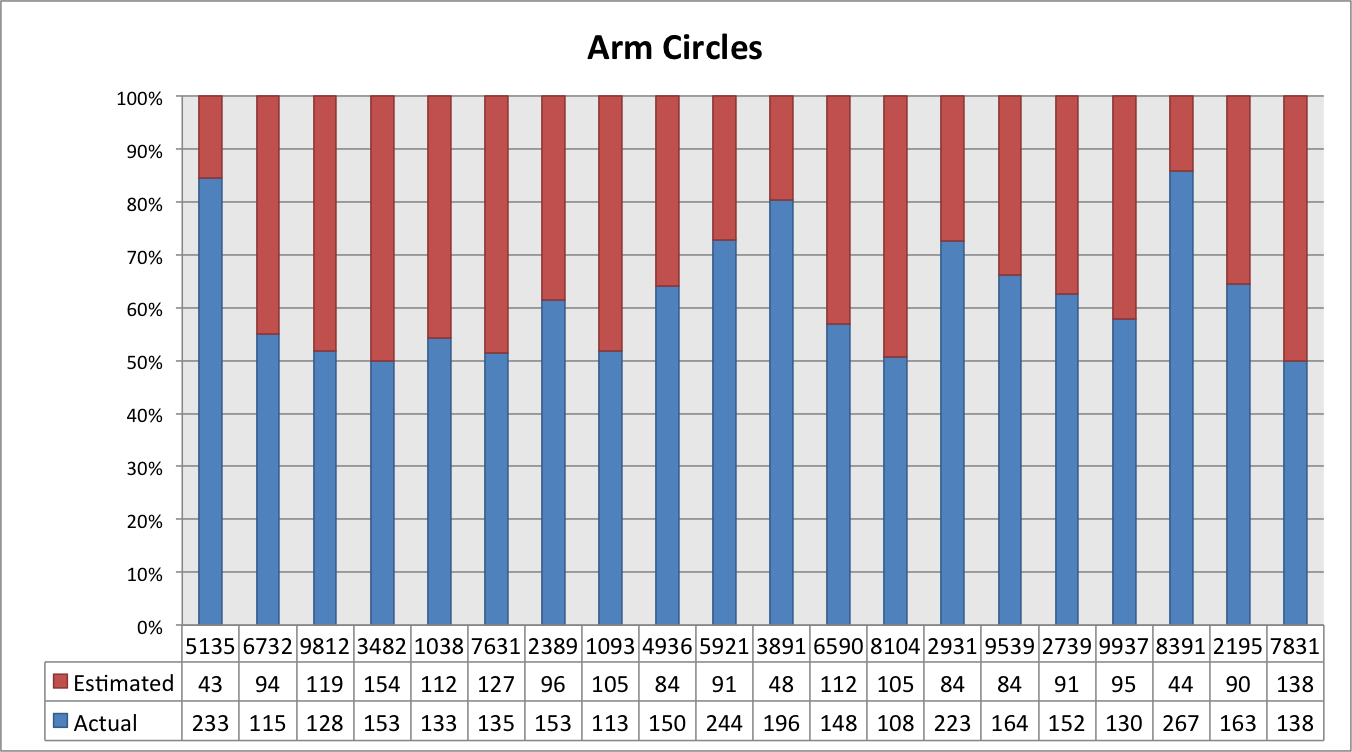
\includegraphics[width=0.5\textwidth]{images/armcircles}
\caption{Arm Circles Results}
\end{figure}
\begin{figure}[htp]
	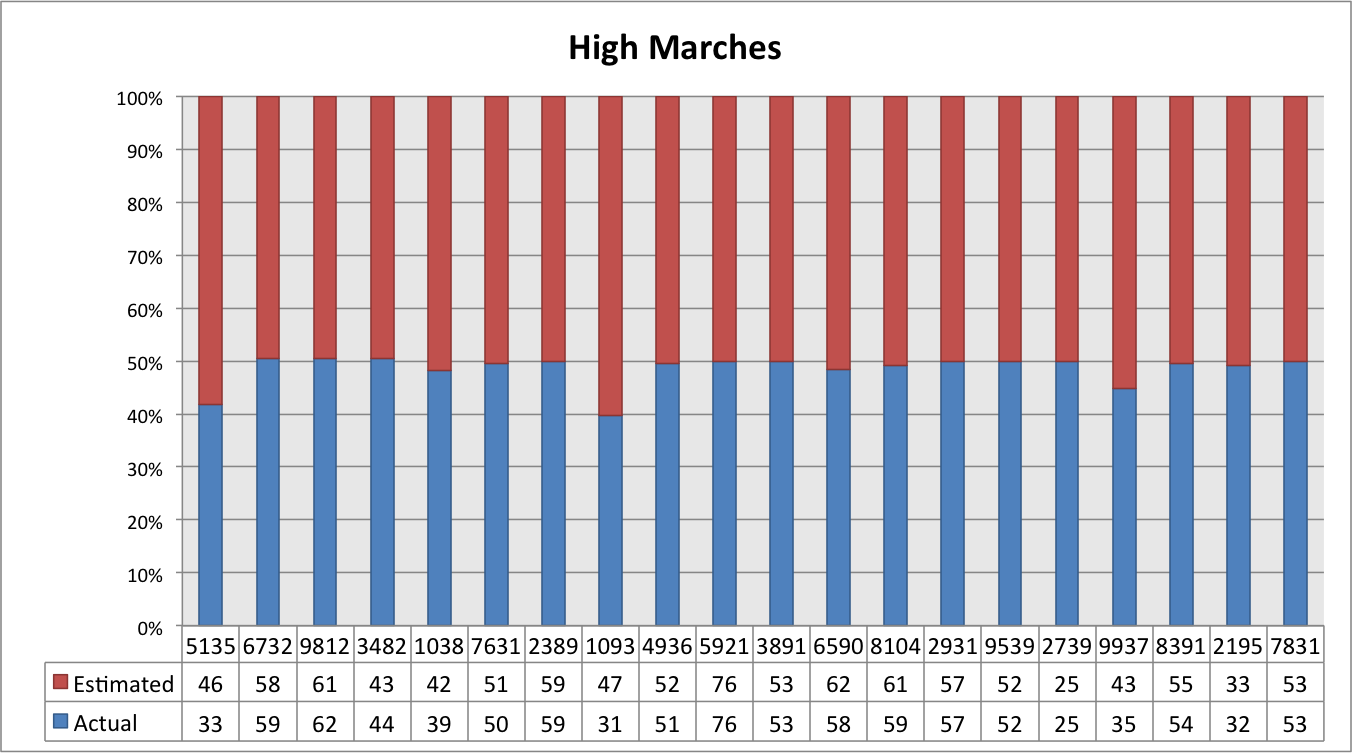
\includegraphics[width=0.5\textwidth]{images/highmarches}
\caption{High Marches Results}
\end{figure}
\begin{figure} [htp]
	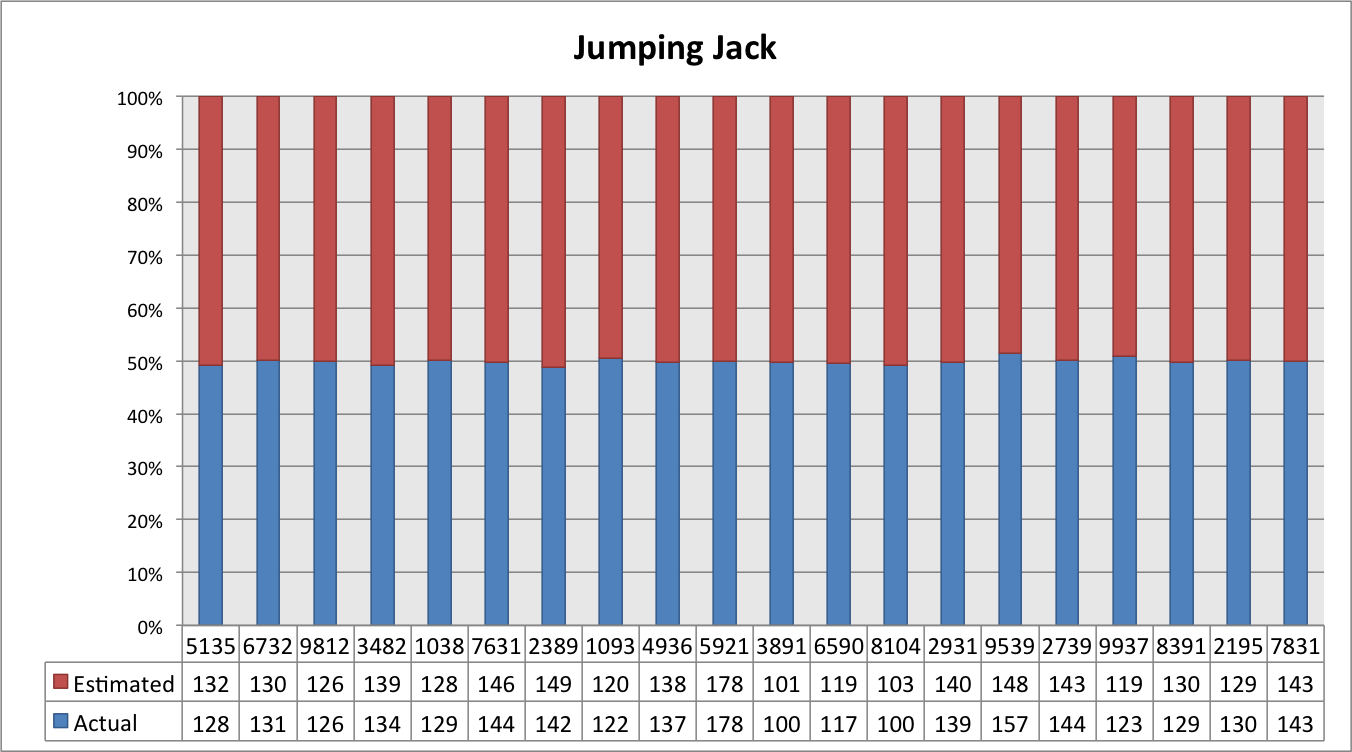
\includegraphics[width=0.5\textwidth]{images/jumpingjack}
\caption{Jumping Jacks Results}
\end{figure}
\begin{figure} [htp]
	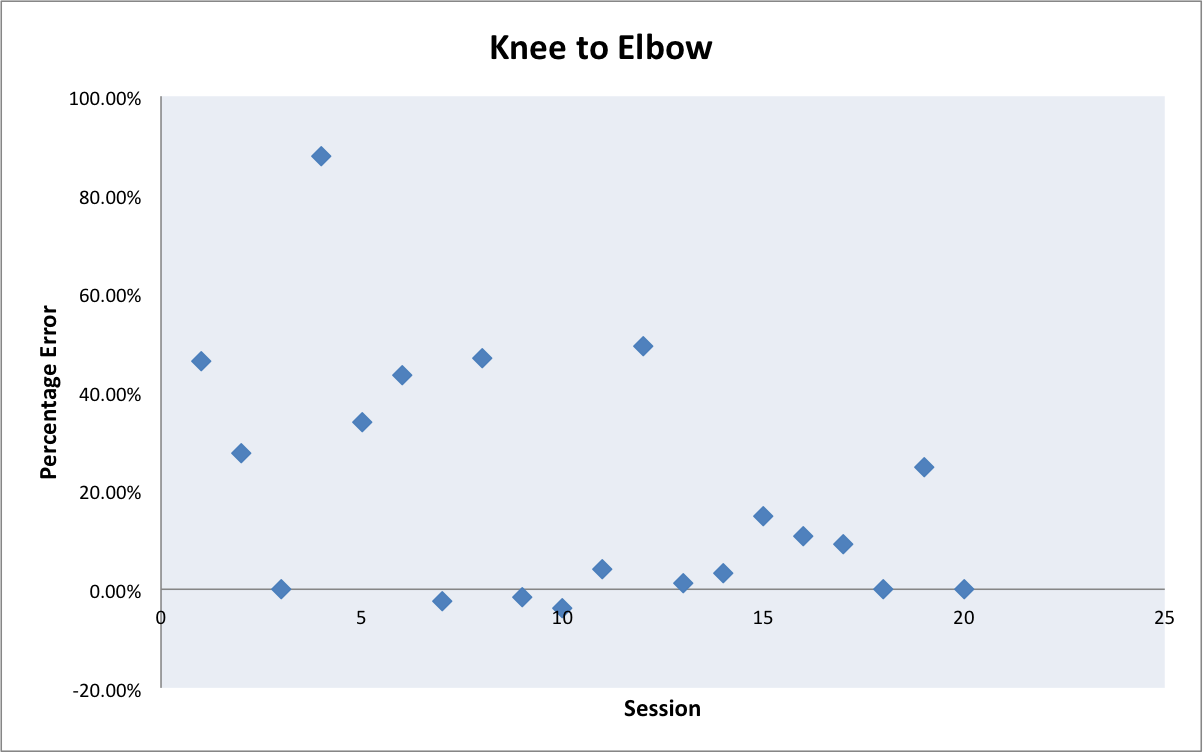
\includegraphics[width=0.5\textwidth]{images/kneetoelbow}
\caption{Knee to Elbow Results}
\end{figure}
\begin{figure} [htp]
	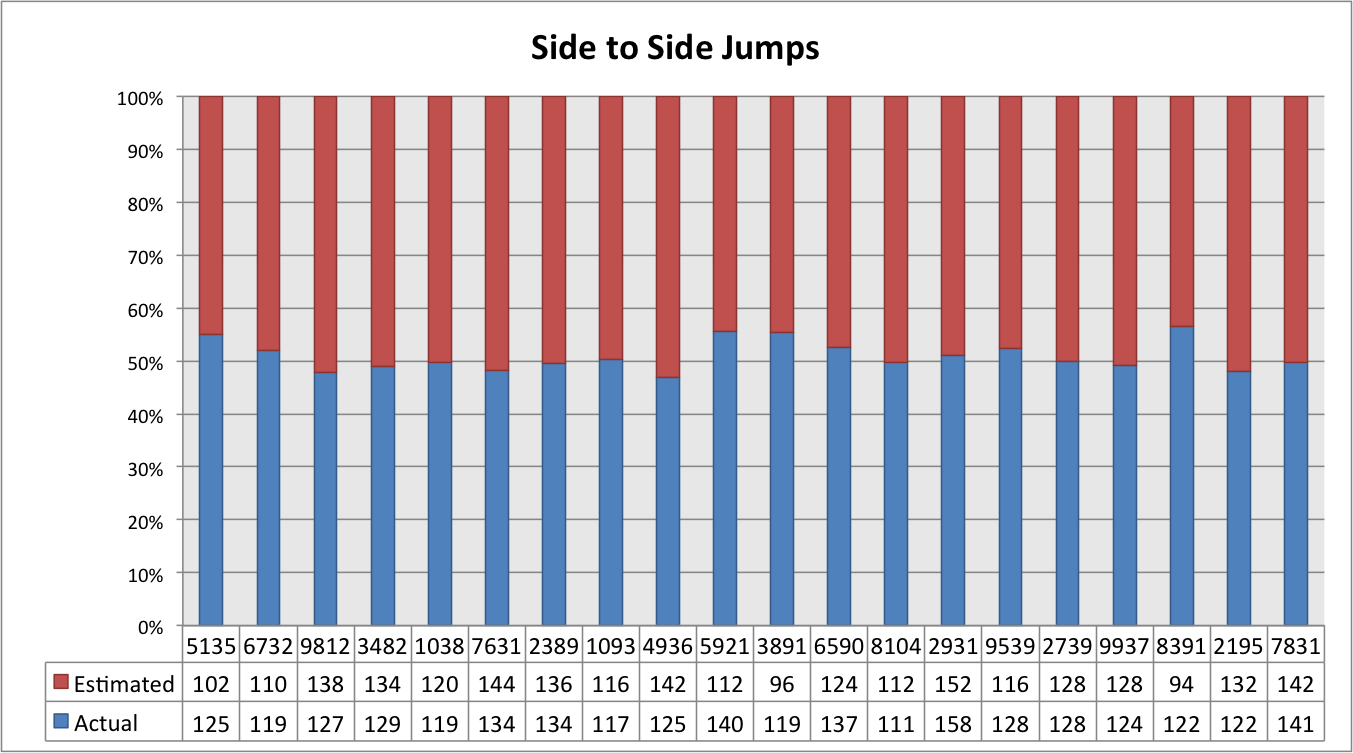
\includegraphics[width=0.5\textwidth]{images/sidetoside}
\caption{Side to Side Results}
\end{figure}
\begin{figure} [htp]
	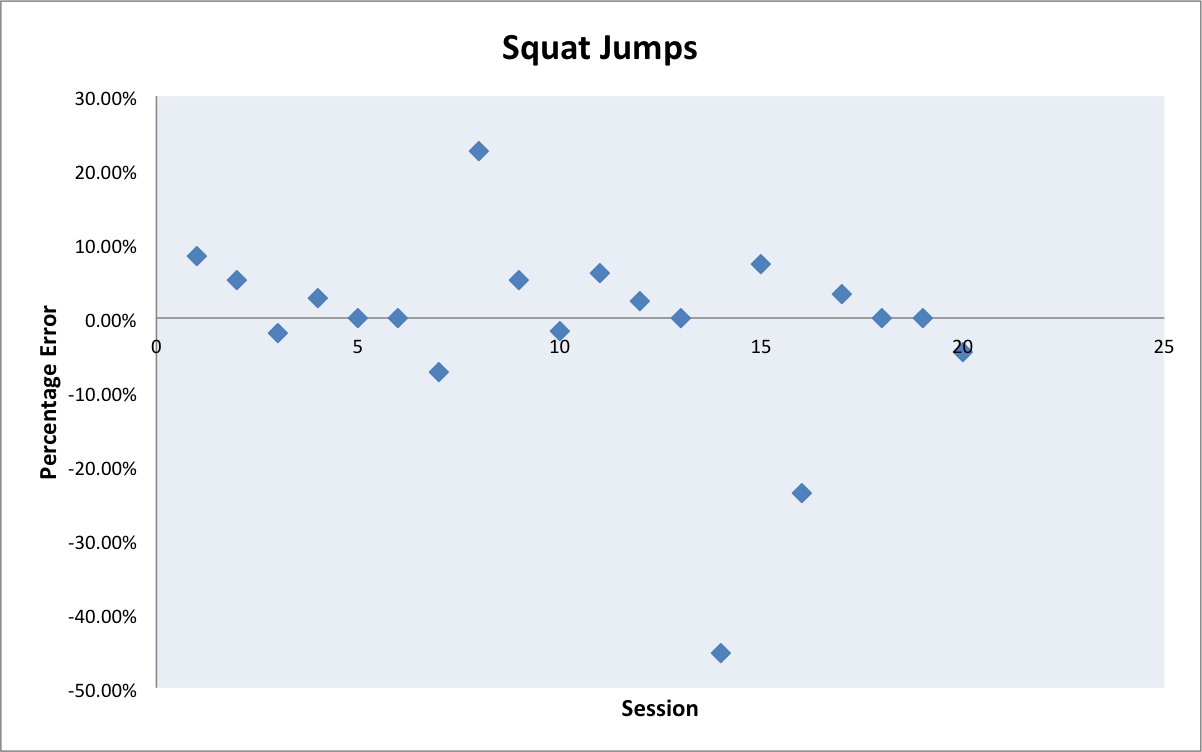
\includegraphics[width=0.5\textwidth]{images/squatjumps}
\caption{Squat Jumps Results}
\end{figure}
\begin{figure} [h!]
	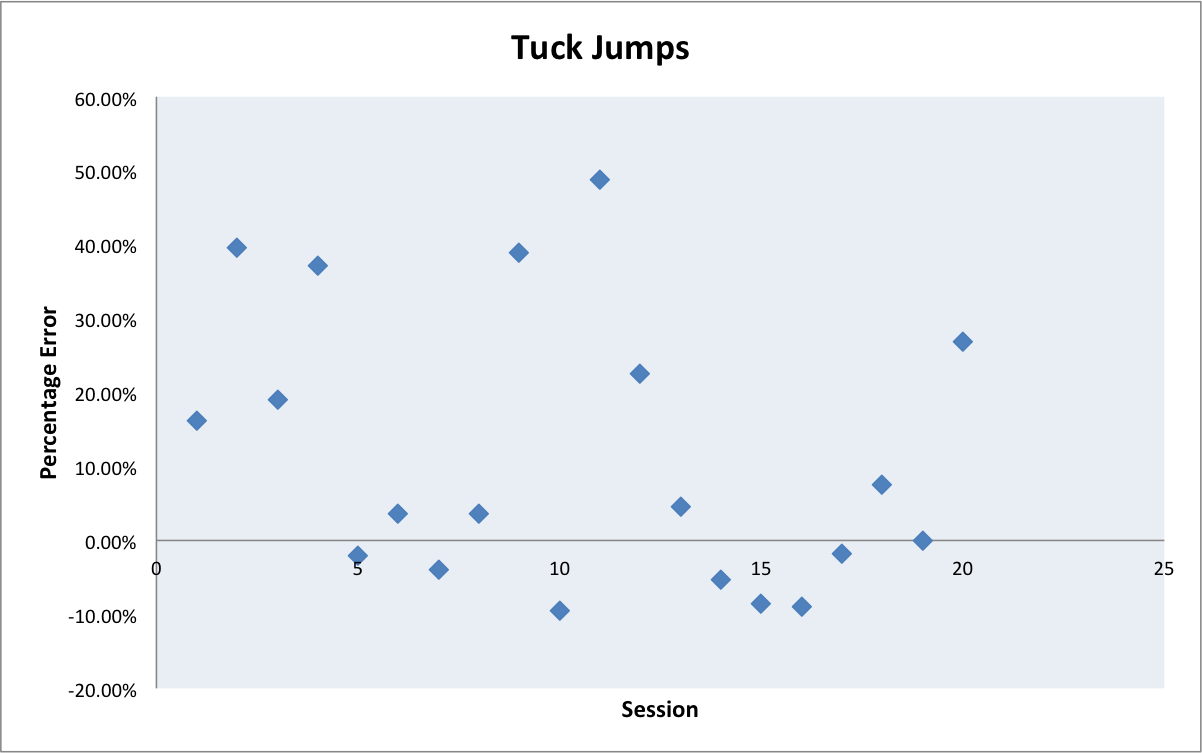
\includegraphics[width=0.5\textwidth]{images/tuckjumps}
\caption{Tuck Jumps Results}
\end{figure} 
Clearly, our model gave more accurate count estimates for certain exercise (such as jumping jacks) and less accurate estimates for others (such as arm circles). Another observation we can make is that the bias in our model is not random but tends to either overestimate most of the time or underestimate most of the time. A discussion of the possible explanations for the performance disparities and inaccuracies is left for the Discussion section. \\